\section{543 --- Diameter of Binary Tree}
Given a binary tree, you need to compute the length of the diameter of the tree. The diameter of a binary tree is the length of the longest path between any two nodes in a tree. This path may or may not pass through the root.

\paragraph{Example:}
\begin{flushleft}
\textbf{Input}:

\begin{figure}[H]
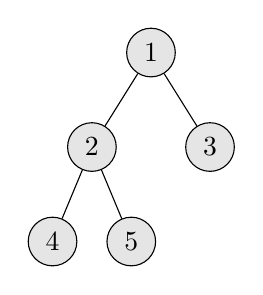
\begin{tikzpicture}
[every node/.style={draw, circle, fill=gray!20!, minimum size=5mm},
level 2/.style ={sibling distance=1cm}, 
level 3/.style={sibling distance=8mm},
level distance=1.2cm]
\node{1}
 child {node{2} child {node{4}} child {node{5}}}
 child {node{3}};
\end{tikzpicture}
\end{figure}

\textbf{Output}: 3, which is the length of the path $[4,2,1,3]$ or $[5,2,1,3]$.
\end{flushleft}
\paragraph{Note:} 
\begin{itemize}
\item The length of path between two nodes is represented by the number of edges between them. 
\end{itemize}